\documentclass[tikz,dvipsnames]{standalone}
\usepackage[utf8]{inputenc}
\usepackage[]{xcolor}
\PassOptionsToPackage{dvipsnames}{xcolor}
\usepackage{amsmath}
\usepackage{amssymb}

\usetikzlibrary{arrows,positioning,shapes}
\usetikzlibrary{decorations.pathreplacing,decorations.markings}
\usetikzlibrary{calc}
% https://tex.stackexchange.com/questions/3161/tikz-how-to-draw-an-arrow-in-the-middle-of-the-line
\tikzset{
  % style to apply some styles to each segment of a path
  on each segment/.style={
    decorate,
    decoration={
      show path construction,
      moveto code={},
      lineto code={
        \path [#1]
        (\tikzinputsegmentfirst) -- (\tikzinputsegmentlast);
      },
      curveto code={
        \path [#1] (\tikzinputsegmentfirst)
        .. controls
        (\tikzinputsegmentsupporta) and (\tikzinputsegmentsupportb)
        ..
        (\tikzinputsegmentlast);
      },
      closepath code={
        \path [#1]
        (\tikzinputsegmentfirst) -- (\tikzinputsegmentlast);
      },
    },
  },
  % style to add an arrow in the middle of a path
  mid arrow/.style={postaction={decorate,decoration={
        markings,
        mark=at position .5 with {\arrow[#1]{stealth}}
      }}},
  % style to add an arrow at a position of a path
  arrow at/.style 2 args={postaction={decorate,decoration={
        markings,
        mark=at position #1 with {\arrow[#2]{stealth}}
      }}},
}

\tikzset{cross/.style={cross out, draw=black, minimum size=2*(#1-\pgflinewidth), inner sep=0pt, outer sep=0pt},
%default radius will be 1pt. 
cross/.default={1pt}}

%color
\colorlet{TopOp1}{RedOrange}
\colorlet{TopOp2}{JungleGreen!60!black}
\colorlet{TopOp3}{Mulberry}
\DeclareMathOperator{\Obj}{Obj}
\DeclareMathOperator{\Hom}{Hom}

\usetikzlibrary{knots}
\begin{document}
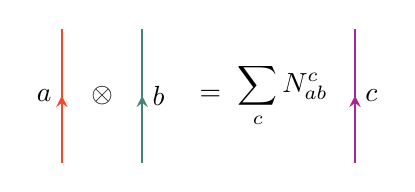
\begin{tikzpicture}[thick,scale=1.7]
  \pgfmathsetmacro{\sep}{.3}
  \draw[postaction={on each segment={mid arrow}},color=TopOp1] (0,0) --node[midway,anchor=east,black] {$a$}  ++(0,1);
  \draw[postaction={on each segment={mid arrow}},color=TopOp2] (2*\sep,0) --node[midway,anchor=west,black] {$b$}  ++(0,1);
  \node at (\sep,.5) {$\displaystyle\otimes$};
  \node at (3.7*\sep,.5) {$=$};
  \node at (5.5*\sep,.5) {$\displaystyle\sum_{c}N_{ab}^c$};
  \draw[postaction={on each segment={mid arrow}},color=TopOp3] (7.3*\sep,0) --node[midway,anchor=west,black] {$c$}  ++(0,1);

\end{tikzpicture}
\end{document}
